\chapter{Context}
\label{chap:context}

\section{Background on PAKEs}
\subsection{What Problem Do PAKEs Solve?}
In the modern day when you login to a website a \gls{tls} encrypted channel is established, over which your password is sent in plaintext.
The server then computes the hash of your password, sometimes with a salt or some other additional data.
This hash is then compared with whatever is stored in the server's database for your account, and access is granted based on whether the hash matched.

This approach is fundamentally flawed, allowing the plaintext password to leave your device gives attackers many more opportunities at which they can steal your password.
Be that from compromising the \gls{tls} channel via a \gls{downgrade-attack} or by malware on the server intercepting your password as the server processes it.

\glspl{pake} solve this problem in a fundamentally different way, and they have many benefits because of this.
Namely with \glspl{pake} your password never leaves your device, it is used to calculate a secret key which is shared with the server.
Another property of how \glspl{pake} are constructed is that you and the server are both \enquote{authenticated} with each other once you acquire the shared key.
This is in contrast with the approach of \gls{tls} and certificates, where only the server is authenticated.

% Horizontal version
\begin{figure}[H]
  \centering
  \begin{tikzpicture}[thick,>=latex]
    \node[alice,minimum size=1.5cm] at (0,0) {Alice -- Client};
    \node[bob,mirrored,minimum size=1.5cm] at (5,0) {Bob -- Server};
    \draw[->] (1,0.5) -- (4,0.5) node[midway, above] {password};
    \draw[->] (4,-0.5) -- (1,0-0.5) node[midway, above] {auth \cmark};

    \node[alice,minimum size=1.5cm] at (9,0) {Alice -- Client};
    \node[bob,mirrored,minimum size=1.5cm] at (14,0) {Bob -- Server};
    \node at (10.3,0.8) {password};
    \draw[->] (10, 0.5) -- (10,-0.5) node[midway, right, xshift=0.1cm, yshift=0.1cm, scale=0.05] {
\includegraphics{wand.png}};
    \node[scale=0.02] at (10.3,-0.7) {
\includegraphics{key.png}};
    \node at (12.8,0.8) {verifier};
    \draw[->] (13, 0.5) -- (13,-0.5) node[midway, left, xshift=-0.1cm, yshift=0.1cm, scale=0.05] {
\includegraphics{wand.png}};
    \node[scale=0.02] at (12.5,-0.7) {
\includegraphics{key.png}};
    \draw[<->] (10.8,-0.7) -- (12,-0.7) node[midway, below] {auth \cmark};

    \draw (7,1.3) -- (7,-2.3);
    \draw (2.5,-2) node {Traditional};
    \draw (11.5,-2) node {PAKE};
  \end{tikzpicture}

  \caption{An illustration of the difference traditional password based authentication and \glspl{pake}}
  \label{fig:tls-vs-pake}
\end{figure}

\clearpage
\subsection{What Is a PAKE?}
\glspl{pake} are interactive, two party cryptographic protocols where each party shares knowledge of a password (a low entropy secret) and seeks to obtain a strong shared key e.g. for use later with a symmetric cipher. Critically an eavesdropper who can listen to all messages of the key negotiation cannot learn enough information to bruteforce the password. Another way of phrasing this is that brute force attacks on the key must be \enquote{\glslink{ocrypto}{online}}.

There are two main types of \gls{pake} algorithm -- \glspl{apake} and \glspl{bpake}.
\begin{itemize}
  \item \glspl{bpake} are \glspl{pake} where both parties share knowledge of the same secret password.
  \item \glspl{apake} are \glspl{pake} where one party has the password and the other has a \enquote{\gls{veri}} which is computed via a one-way function from the secret password.
\end{itemize}

% Vertical version
% \begin{figure}[H]
%   \centering
%   \begin{tikzpicture}
%     \node[alice,minimum size=3cm] at (0,0) {Alice -- Client};
%     \node[bob,mirrored,minimum size=3cm] at (10,0) {Bob -- Server};
%     \node[scale=0.05] at (2,1) {
\includegraphics{key.png}};
%     \node[scale=0.05] at (8,1) {
\includegraphics{key.png}};
% 
%     \node[alice,minimum size=3cm] at (0,-7) {Alice -- Client};
%     \node[bob,mirrored,minimum size=3cm] at (10,-7) {Bob -- Server};
%     \node[scale=0.05] at (2,-6) {
\includegraphics{key.png}};
%     \node[scale=0.05] at (8,-6) {
\includegraphics{shuffled_key.png}};
% 
%     \draw (-2,-3.5) -- (12,-3.5);
%     \draw (5,2) node {Balanced PAKE};
%     \draw (5,-5) node {Augmented PAKE};
%   \end{tikzpicture}
% 
%   \caption{An illustration of the difference between \glspl{pake} and traditional password-based authentication}
%   \label{fig:pake-compare}
% \end{figure}

% % Horizontal version
\begin{figure}[H]
  \centering
  \begin{tikzpicture}
    \node[alice,minimum size=1.5cm] at (0,0) {Alice};
    \node[scale=0.03] at (1,0.5) {
\includegraphics{key.png}};
    \node[bob,mirrored,minimum size=1.5cm] at (5,0) {Bob};
    \node[scale=0.03] at (4,0.5) {
\includegraphics{key.png}};

    \node[alice,minimum size=1.5cm] at (7,0) {Alice};
    \node[scale=0.03] at (8,0.5) {
\includegraphics{key.png}};
    \node[bob,mirrored,minimum size=1.5cm] at (12,0) {Bob};
    \node[scale=0.03] at (11,0.5) {
\includegraphics{shuffled_key.png}};

    \draw (6,1.3) -- (6,-2.3);
    \draw (2.5,-2) node {Balanced PAKE};
    \draw (9.5,-2) node {Augmented PAKE};
  \end{tikzpicture}

  \caption{An illustration of the difference between \glspl{apake} and \glspl{bpake}}
  \label{fig:pake-compare}
\end{figure}

\subsection{How Can PAKEs Thwart the Effectiveness of Quantum Computers?}
With quantum computing advancing ever faster, classical cryptography systems such as those based on the hardness of the factoring problem\footnote{Finding $p,$ given $N = p * q$ where $p$ and $q$ are large prime numbers.} (\gls{rsa}), or the discrete-logarithm problem\footnote{Finding $a$ given $g^a mod p$ for large $a$ and prime $p$} (\gls{dh}, \gls{ecdh}) are increasingly coming into question as quantum computers can solve these problems efficiently.
During the \gls{cfrg}'s recent \gls{pake} standardisation efforts a new property of \glspl{pake} emerged called \enquote{quantum annoying}.
In their paper \citetitle{quantum-annoying} \cite{quantum-annoying}, \citeauthor{quantum-annoying} define the \enquote{quantum annoying} property of \glspl{pake} as a scheme where a quantum computer can compromise a scheme, but that solving one discrete logarithm problem only gives one guess at the password.
This makes \glspl{pake} incredibly attractive as stopgap solution giving researchers a few more vital years to research and test post-quantum cryptography.
The need for these years of research was made painfully clear by \textcite{break-sidh} when they recently broke the \gls{sidh} post-quantum cryptography scheme.

\clearpage

\subsection{A Brief History of PAKE Algorithms}
The first \gls{pake} algorithm was Bellovin and Merritt's \gls{eke} scheme \cite{eke}.
It works using a mix of \gls{symcrypto} and \gls{asymcrypto} to perform a key exchange.
This comes with many challenges and subtle mistakes that are easy to make;
primarily for the security of the system whatever is encrypted by the shared secret key(P) must be indistinguishable from random data.
Otherwise an attacker can determine whether their guess at a trial decryption is valid.
The \gls{rsa} variant of \gls{eke} has this issue -- the \gls{rsa} parameter $e$ is what is encrypted and sent in the first message.
For \gls{rsa} all valid values of $e$ are odd, so this would prevent it being used.
This is solved by adding $1$ to $e$ with a $50\%$ chance.
\Cref{fig:eke-rsa} shows this protocol in full. While many of the initial variants on \gls{eke} have been shown to flawed/vulnerable, later variants have made it into real world use, such as in \gls{eap} \cite{eap} where it is available as \gls{eap}-\gls{eke} \cite{eap-eke}.
In \cref{chap:appendix-eke} you can find a Python implementation of this scheme.

\subsubsection{An Aside on Notation}
\begin{itemize}
  \item $\shortleftarrow$: Assignment -- $x \shortleftarrow \ 5$ means x is assigned a value of 5.
  \item $\cryptoSample$: Sampling from a given set -- $x \cryptoSample \ \mathbb{R}$ means to choose $x$ at random from the set of real numbers.
  \item $||$: Concatenation -- $x || y$ means $x$ concatenated with $y$.
\end{itemize}

\begin{center}
  \captionof{table}{\gls{eke} shared parameters}
  \begin{tabular}{ ccl }
    \toprule
    Shared Parameter & Secret & Explanation \\
    \midrule
    $P$ & yes & the shared password \\
    \bottomrule
  \end{tabular}
\end{center}

\begin{figure}[H]
  \pseudocodeblock[head=EKE-RSA]{
    \textbf{Alice} \< \< \textbf{Bob} \\[0.1\baselineskip][\hline]
    \< \< \\[-0.5\baselineskip]
    Ea \gets (e, n) \< \< \\
    b \sample \bin \< \sendmessageright*{A,P(e + b),n} \< Ea \gets (e, n)\\ 
    challenge_A \sample \ZZ_n \< \sendmessageleft*{P(Ea(R))} \< R \sample \text{Keyspace}\\ 
    \< \sendmessageright*{R(challenge_A)} \< challenge_B \sample \ZZ_n \\
    \text{verify } challenge_A \< \sendmessageleft*{R(challenge_A, challenge_B)} \< \\
    \< \sendmessageright*{R(challenge_B)} \< \text{verify } challenge_B
  }

  \caption{Implementing \gls{eke} using \gls{rsa}}
  \label{fig:eke-rsa}
\end{figure}

\clearpage

\subsubsection{SPAKE}
\glslink{spake}{SPAKE1} and \glslink{spake}{SPAKE2} are \glspl{bpake} which were introduced slightly later on by \citeauthor{spake} \cite{spake} as variations on \gls{eke}.
They are very similar so we will just explore \glslink{spake}{SPAKE2} as we are more interested in \glslink{ocrypto}{online} algorithms.
\gls{spake} differs from EKE in the following ways:

\begin{enumerate}
  \item The encryption function is replaced by a simple one-time pad.
  \item The \gls{asymcrypto} is provided by \gls{dh}
  \item There is no explicit mutual authentication phase where challenges are exchanged.
    This has the advantage of reducing the number of messages that need to be sent.
\end{enumerate}

\begin{center}
  \rowcolors{0}{}{mintbg}
  \captionof{table}{\gls{spake} shared parameters}
  \begin{tabularx}{\linewidth}{ ccX }
    \toprule
    Shared Parameter & Secret & Explanation \\
    \midrule
    $pw$ & yes & the shared password encoded as an element of $\ZZ_p$ \\
    $\GG$ & no & the mathematical group in which we will perform all operations \\ 
    $g$ & no & the generator of $\GG$ \\
    $p$ & no & the \gls{safeprime} which defines the finite field for all operations in $\GG$ \\
    $M$ & no & an element in $\GG$ associated with user $A$ \\
    $N$ & no & an element in $\GG$ associated with user $B$ \\
    $H$ & no & a secure hash function \\
    \bottomrule
  \end{tabularx}
\end{center}

\begin{figure}[H]
  \pseudocodeblock[head=SPAKE2]{
    \textbf{Alice} \< \< \textbf{Bob} \\[0.1\baselineskip][\hline]
    \< \< \\[-0.5\baselineskip]
    x \sample \ZZ_p \< \< y \sample \ZZ_p \\
    X \gets g^x \< \< Y \gets g^y \\
    X^* \gets X \cdot M^{pw} \< \< Y^* \gets X \cdot N^{pw} \\
    \< \sendmessageright*{X^*} \< \\
    \< \sendmessageleft*{Y^*} \< \\
    K_A \gets (Y^* / N^{pw})^x \< \< K_B \gets (X^* / M^{pw})^y \\
    SK_A \gets H(A, B, X^*, Y^*, Ka) \< \< SK_B \gets H(A, B, X^*, Y^*, Kb)
  }

  \caption{SPAKE2 Protocol}
  \label{fig:spake2}
\end{figure}

\clearpage

\subsubsection{SRP}
Finally we will look at \gls{srp} an \gls{apake} first published in 1998, unlike \glslink{spake}{SPAKE2} it is not a modification of \gls{eke}.
\gls{srp} has gone through many revisions, at time of writing \glslink{srp}{SRP6a} is the latest version.
\gls{srp} is likely the most used \gls{pake} protocol in the world due to it's use in Apple's iCloud Keychain \cite{apple-keychain-srp} and it's availability as a \gls{tls} ciphersuite \cite{tls-srp}.
However it is quite weird for what it does and there is no security proof for it \cite{srp-blog}. An implementation of the protocol in Python can be found in \cref{chap:appendix-srp}.

\begin{center}
  \rowcolors{0}{}{mintbg}
  \captionof{table}{\gls{srp} parameters}
  \begin{tabularx}{\linewidth}{ ccX }
    \toprule
    Parameter & Secret & Explanation \\
    \midrule
    $v$ & yes & the \gls{veri}\label{text:srp-verifier-generation} stored by the server: $v=g^{H(s,I,P)}$ \\
    $P$ & yes & the user's password \\
    $I$ & no & the user's name \\
    $g$ & no & the generator of $\GG$ \\
    $p$ & no & the \gls{safeprime} which defines the finite field for all operations in $\GG$ \\
    $H$ & no & a secure hash function \\
    \bottomrule
  \end{tabularx}
\end{center}

\begin{figure}[H]
  \pseudocodeblock[head=SRP]{
    \textbf{Alice} \< \< \textbf{Bob} \\[0.1\baselineskip][\hline]
    \< \< \\[-0.5\baselineskip]
    a \sample \{1 \dots n - 1\} \< \sendmessageright*{I} \< s,v \gets \text{lookup}(I)\\
    x \gets H(s, I, P) \< \sendmessageleft*{s} \< b \sample \{1 \dots n - 1\}\\
    A \gets g^a \< \sendmessageright*{A} \< B \gets 3v + g^b \\
    u \gets H(A, B) \< \sendmessageleft*{B} \< u \gets H(A, B)\\
    S \gets (B - 3g^x)^{a+ux}\< \< S \gets (Av^u)^b\\
    M_1 \gets H(A,B,S) \< \sendmessageright*{M_1} \< \text{verify } M_1\\
    \text{verify } M_2 \< \sendmessageleft*{M_2} \< M_2 \gets H(A,M_1,S)\\
    K \gets H(s)\< \< K \gets H(S)
  }

  \caption{SRP-6 Protocol}
  \label{fig:srp}
\end{figure}

\clearpage

\section{Elliptic Curve Cryptography}
Many modern cryptographic protocols make use of a mathematical object known as an elliptic curve.
First proposed for use in cryptography in 1985 independently by Neal Koblitz \cite{ecc-first-use-koblitz} and Victor S. Miller \cite{ecc-first-use-miller}.
Elliptic curves are attractive to cryptographers as they maintain a very high level of strength at smaller key sizes, this allows for protocols to consume less bandwidth, less memory and execute faster \cite{state-of-ecc}.
To illustrate just how great the size savings are -- \gls{nist} suggests that an elliptic curve key of just 256 bits provides the same level of security as an \gls{rsa} key of 3072 bits \cite{nist-ecc-reqs}.

\subsection{But What Actually Is an Elliptic Curve?}
With regards to cryptography elliptic curves tend to come in one of two forms:
\begin{itemize}
  \item Short Weierstra\ss{} Form: $y^2 = x^3 + ax + b$
  \item Montgomery Form: $by^2 = x^3 + ax^2 + x$
\end{itemize}

\begin{figure}[H]
  \centering
  \begin{tikzpicture}[thick,>=latex]
    \begin{scope}
      \draw[<->,gray] (-3,0) -- (3,0) node[right] {$x \in \mathbb{R}$};
      \draw[<->,gray] (0,-3) -- (0,3) node[above] {$y \in \mathbb{R}$};
      \draw[thick, name path=curve, every plot/.style={smooth}] plot[id=weierstrass-curve-1, raw gnuplot] function {
        f(x,y) = y**2 - (x**3 - 2.5*x + 1);
        set xrange [-3:3];
        set yrange [-3:3];
        set view 0,0;
        set isosample 50,50;
        set cont base;
        set cntrparam levels incre 0,0.1,0;
        unset surface;
        splot f(x,y);
      };
    \end{scope}

    \node at (0,-4) {$y^2 = x^3 - 2 x - 1$ over $\mathbb{R}$};
    \node at (0,-5) {Short Weierstra\ss{} Form};

    \begin{scope}[xshift=8cm]
      \draw[<->,gray] (-3,0) -- (3,0) node[right] {$x \in \mathbb{R}$};
      \draw[<->,gray] (0,-3) -- (0,3) node[above] {$y \in \mathbb{R}$};
      \draw[thick, name path=curve, every plot/.style={smooth}] plot[id=montgomery-curve-1, raw gnuplot] function {
        f(x,y) = 2*y**2 - (x**3 - 3*x - x);
        set xrange [-3:3];
        set yrange [-3:3];
        set view 0,0;
        set isosample 50,50;
        set cont base;
        set cntrparam levels incre 0,0.1,0;
        unset surface;
        splot f(x,y);
      };
    \end{scope}

    \node at (8,-4) {$2 y^2 = x^3 - 3 x^2 - x$ over $\mathbb{R}$};
    \node at (8,-5) {Montgomery Form};
  \end{tikzpicture}

  \caption{Elliptic curves over $\RR$, Adapted from TikZ for Cryptographers \cite{tikz-crypto}}
\end{figure}

Weierstra\ss{} form is special as it is the general case for all elliptic curves, meaning all elliptic curves can be expressed as a Weierstra\ss{} curve.
This property means that it is commonly used for expressing various curves.
Montgomery form isn't quite as flexible, however it is favourable because it leads to significantly faster multiplication and addition operations via Montgomery's ladder \cite{montgom-ladder}.

\subsection{How Do We Do Cryptography With Curves?}
To perform cryptography with elliptic curves we need to define an \enquote{\gls{abgroup}} to work in.
An \gls{abgroup} is a group whose group operation is also commutative, for example the addition operator over the integers: ($+$, $\ZZ$) is an \gls{abgroup}.
\glspl{abgroup} form the basis of many modern cryptographic algorithms, a \gls{dh} key exchange can be performed in any \gls{abgroup} for instance.

Our \gls{abgroup} is built on the idea of \enquote{adding} points on the curve.
To add two points, we find the line which passes through our two points and we continue along that line until we hit our curve again.
We then reflect this point in the $x$-axis to get our result.
What if we want to add our point to itself? Now there isn't a unique line through one point, however we are making the rules so in this case we will take the tangent to the curve at that point and then we can treat it the same as before.
What if our line doesn't intersect with the curve? In this case we define a new point called the \enquote{neutral element} -- $\mathcal{O}$.
It is also called the point at infinity as it can be considered to be the single point at the end of every vertical line at infinity.
\Cref{fig:point-add-rules} illustrates all of these rules and edge cases.

\begin{figure}[H]
  \centering
  \begin{tikzpicture}[scale=.555]

    \begin{scope}[xshift=0cm]
      \plotcurve{-2}{2}
      \draw[->, >=latex, thick] (-2.5,-1) -- ++(0,3.5) node[right] {$\mathcal{O}$};
      \node[below] at (0,-4) {Neutral element $\mathcal{O}$};
    \end{scope}

    \begin{scope}[xshift=7.5cm]
      \plotcurve{-2}{2}
      \draw[dashed, semithick, name path=vertical] (-1.25,2.5) -- ++(0,-5);
      \draw[name intersections={of=curve and vertical}] (intersection-1) node {$\bullet$} node[above left] {$P$}
      (intersection-2) node {$\bullet$} node[below left] {$-P$};
      \node[below] at (0,-4) {Inverse element $-P$};
    \end{scope}

    \begin{scope}[xshift=15cm]
      \plotcurve{-2}{2}
      \draw[thick, name path=chord] (-2.5,.5) -- (2.5,2.0);
      \draw[name intersections={of=curve and chord}] (intersection-1) node {$\bullet$} node[above left] {$P$}
      (intersection-2) node {$\bullet$} node[above right=-1pt] {$Q$}
      (intersection-3) node {$\bullet$} coordinate[name=mPQ];
      \draw[dashed, semithick, name path=vertical] (mPQ) ++(0,1) -- +(0,-5.5);
      \draw[name intersections={of=curve and vertical}] (intersection-2) node {$\bullet$} node[below left] {$P+Q$};
      \node[below, align=center] at (0,-4) {Addition $P+Q$ \\ ``Chord rule''};
    \end{scope}

    \begin{scope}[xshift=22.5cm]
      \plotcurve[thick, tangent=0.265, every plot/.style={sharp plot}]{-2}{2}
      \draw[thick, use tangent, name path=chord] (-.6,0) -- (1.5,0);
      \draw[name intersections={of=curve and chord}] (intersection-1) node {$\bullet$} node[above] {$P$}
      (intersection-2) node {$\bullet$} coordinate[name=mPQ];
      \draw[dashed, semithick, name path=vertical] (mPQ) ++(0,1) -- +(0,-5.0);
      \draw[name intersections={of=curve and vertical}] (intersection-2) node {$\bullet$} node[below left] {$2P$};
      \node[below, align=center] at (0,-4) {Doubling $P+P$ \\ ``Tangent rule''};
    \end{scope}

  \end{tikzpicture}
  \caption{Elliptic Curve Group Operations, reproduced from TikZ for Cryptographers \cite{tikz-crypto}}
  \label{fig:point-add-rules}
\end{figure}

However it's not quite that simple for us. We cannot use $\RR$ as computers only have finite resources we need a finite set to work in. Instead we define our operations over a \gls{ff}, we will use the \gls{ff} of the integers mod a prime, denoted $\ZZ_p$ for some prime $p$. Lets take a look at what our finite fields look like in a small finite field -- $\ZZ_{89}$. \begin{figure}[H]
  \centering

  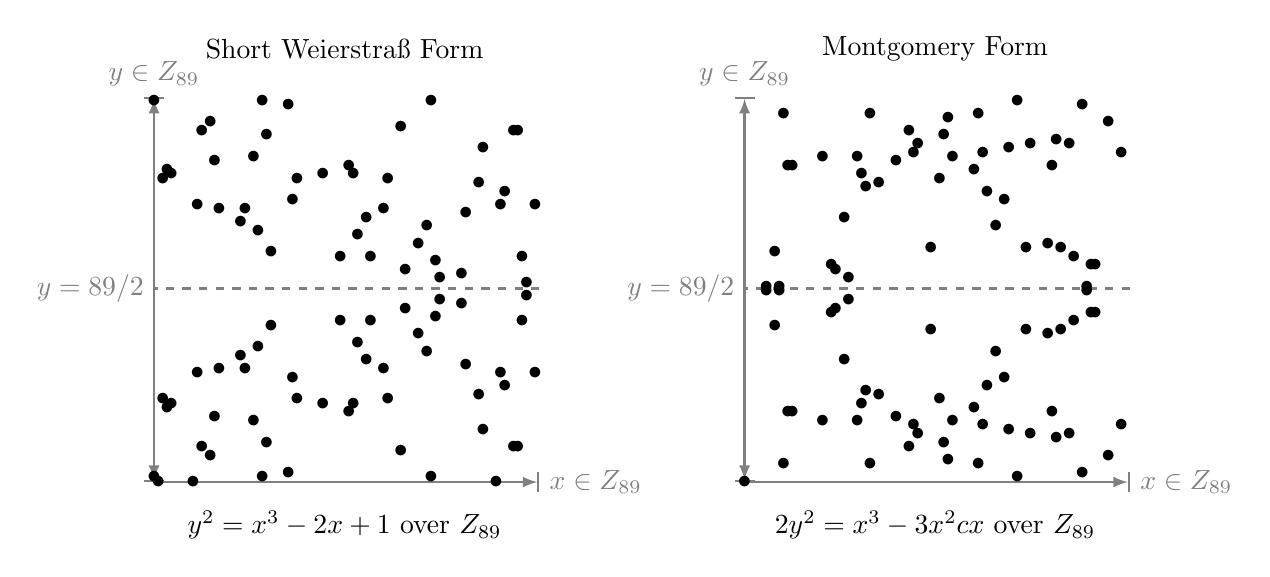
\begin{tikzpicture}[thick,>=latex]
    % Generate list of points with Sage:
    % sage: E = EllipticCurve(Integers(89), [-2,1])
    % sage: points = {tuple(p)[:2] for p in E.points()}
    % sage: print(points)
    \begin{scope}[scale=.055]
      \draw[|<->|,gray] (0,0) -- (0,89) node[above] {$y \in \mathbb{Z}_{89}$};
      \draw[->|,gray] (0,0) -- (89,0) node[right] {$x \in \mathbb{Z}_{89}$};
      % weirdness to make the line actually split the plane
      \draw[dashed,gray] (89,44.7) -- (0,44.7) node[left] {$y = 89/2$};
      \foreach \point in {
        (43, 37), (50, 52), (72, 27), (20, 29), (58, 40), (58, 49), (14, 15), (27, 36), (13, 83), (26, 80), (47, 57), (65, 38), (3, 72), (3, 17), (24, 58), (33, 70), (26, 9), (84, 8), (54, 19), (45, 16), (85, 52), (14, 74), (4, 18), (75, 69), (45, 73), (65, 51), (86, 46), (49, 61), (33, 19), (81, 22), (39, 71), (25, 88), (9, 0), (79, 0), (50, 37), (2, 70), (53, 63), (20, 60), (27, 53), (39, 18), (84, 81), (31, 87), (43, 52), (80, 25), (1, 0), (25, 1), (15, 63), (76, 12), (64, 1), (63, 30), (66, 47), (80, 64), (83, 8), (72, 62), (88, 25), (2, 19), (21, 63), (23, 14), (21, 26), (64, 88), (32, 65), (71, 48), (88, 64), (81, 67), (10, 25), (31, 2), (0, 88), (85, 37), (66, 42), (61, 55), (53, 26), (71, 41), (10, 64), (11, 8), (75, 20), (11, 81), (32, 24), (54, 70), (15, 26), (49, 28), (0, 1), (83, 81), (57, 7), (86, 43), (46, 71), (24, 31), (23, 75), (4, 71), (47, 32), (76, 77), (13, 6), (63, 59), (46, 18), (61, 34), (57, 82)
      } {\node at \point {$\bullet$};}
      \node at (44, 100) {Short Weierstra\ss{} Form};
      \node at (44,-10) {$y^2 = x^3 - 2 x + 1$ over $\mathbb{Z}_{89}$};
    \end{scope}

    % Generate list of points with Python:
    % >>> f=lambda x,y: (int(2 * y**2) % 89) == ((x**3 -3*(x**2) - x) % 89)
    % >>> # yes this is suspect as fuck but it all works because modular arithmetic 🙃
    % >>> points = {(x,y) for x in range(89) for y in range(89) if f(x,y)}
    % >>> print(points)
    \begin{scope}[xshift=7.5cm,scale=.055]
      \draw[|<->|,gray] (0,0) -- (0,89) node[above] {$y \in \mathbb{Z}_{89}$};
      \draw[->|,gray] (0,0) -- (89,0) node[right] {$x \in \mathbb{Z}_{89}$};
      % weirdness to make the line actually split the plane
      \draw[dashed,gray] (89,44.7) -- (0,44.7) node[left] {$y = 89/2$};
      \foreach \point in {
        (70, 55), (24, 42), (81, 39), (45, 19), (73, 35), (76, 52), (28, 21), (66, 78), (29, 4), (26, 14), (23, 61), (55, 13), (56, 67), (79, 44), (65, 54), (11, 16), (35, 74), (84, 6), (0, 0), (47, 84), (11, 73), (9, 85), (70, 34), (18, 14), (72, 79), (87, 13), (39, 76), (66, 11), (75, 78), (7, 53), (26, 75), (8, 45), (63, 88), (54, 85), (81, 50), (58, 30), (80, 39), (72, 10), (65, 35), (28, 68), (63, 1), (18, 75), (53, 72), (76, 37), (31, 69), (23, 28), (61, 12), (75, 11), (21, 40), (21, 49), (48, 14), (71, 16), (45, 70), (84, 83), (43, 54), (71, 73), (39, 13), (5, 45), (8, 44), (29, 85), (55, 76), (7, 36), (78, 87), (20, 39), (10, 16), (73, 54), (38, 8), (54, 4), (80, 50), (38, 81), (40, 78), (58, 59), (31, 20), (53, 17), (60, 65), (79, 45), (27, 71), (56, 22), (10, 73), (20, 50), (48, 75), (87, 76), (24, 47), (9, 4), (27, 18), (60, 24), (46, 80), (43, 35), (78, 2), (47, 5), (61, 77), (46, 9), (35, 15), (5, 44), (40, 11)
      } {\node at \point {$\bullet$};}
      \node at (44,100) {Montgomery Form};
      \node at (44,-10) {$2y^2 = x^3 - 3x^2 c x$ over $\mathbb{Z}_{89}$};
    \end{scope}
  \end{tikzpicture}

  \caption{Elliptic curves over $\ZZ_{89}$, Adapted from TikZ for Cryptographers \cite{tikz-crypto}}
  \label{fig:ellip-curve-ff}
\end{figure}

\clearpage

This now looks very different to when we were looking at them in $\RR$, however it shows very clearly what the elements of our set look like.
They are points in the 2d coordinate plane with a symmetry around $p/2$.
This might not feel intuitive but it is actually exactly what we should expect to happen, in our finite field when we negate our point's y coordinate, instead of flipping it around the y-axis, our points get wrapped around $y=p$.
Hence our new point is the same distance from $y=p$ as our first point was with $y=0$, this is where our symmetry arises.

\subsection{Where Can Elliptic Curve Cryptography Go Wrong?}
There are many attacks against various aspects of Elliptic Curves, in general they fall into the following categories:
\begin{itemize}
  \begin{item}
    Attacks against the \gls{ecdlp} security of the curve:
    \begin{itemize}
      \item{The rho method \cite{pollard-rho}}
      \item{Transfer Security \cite{multiplicative-transfer-attack,additive-transfer-attack}}
      \item{CM Field Discriminants \cite{safecurves}}
      \item{Curve Rigidity \cite{curve-rigidity}}
    \end{itemize}
  \end{item}
  \begin{item}
    Attacks against the concrete implementation of \gls{ecc}:
    \begin{itemize}
      \item{Ladders required for safe and fast point-scalar multiplication \cite{safecurves}}
      \item{Twist Security \cite{small-subgroup-attack,invalid-curve-attack}}
      \item{Completeness \cite{completeness-attack}}
      \item{Indistinguishability \cite{elligator2}}
    \end{itemize}
  \end{item}
\end{itemize}

All of these attacks individually can weaken or even break the security of a given cryptosystem if not accounted for.
However choosing the right curve is a good step in the right direction and can mitigate many of the attacks listed above.

\section{Modern PAKEs}
Recently many novel \glspl{pake} algorithms have been published, this is partly due to a request from the \gls{ietf} for the \gls{irtf} \gls{cfrg} to carry out a selection process to choose a \gls{pake} for usage in \gls{ietf} protocols.
That process concluded in 2020 with \gls{cpace} and \gls{opaque} being chosen as the recommended \gls{bpake} and \gls{apake} respectively \cite{cfrg-pake-selection-results}.

Some time has passed since this process and we now have some new \glspl{pake} with various interesting properties that are worth taking a look at.

\clearpage

\subsection{CHIP+CRISP}
Introduced in \citeyear{chip+crisp} by \citeauthor{chip+crisp}, CHIP and CRISP are two protocol compilers which instantiate what the authors call an \gls{ipake} \cite{chip+crisp}.
\glspl{ipake} are designed to mitigate the threat of compromising the local storage of a device.
While in the case of \glspl{apake} this is considered for the server side, \glspl{bpake} often require both parties to have knowledge of the plaintext password.
Examples of this include SPAKE-2 \cite{spake} and WPA3's DragonFly/SAE \cite{sae}, both of which require the server and client to have knowledge of the plaintext password.
CHIP+CRISP solves this problem by binding the password to an arbitrary bit-string called the identity, this can be anything, e.g. \enquote{server}, \enquote{router}, \enquote{jonathandata0}.
CHIP and CRISP are both protocol compilers, this means that they aren't themselves protocols but they sit on top of another protocol in order to give that sub-protocol the aforementioned properties, by protecting the underlying data they exchange.

\subsection{KHAPE}
\gls{khape} \cite{khape} is an \gls{apake} from the designers of \gls{opaque}, introduced in \citeyear{khape} it is a variant of \gls{opaque} which doesn't rely on the use of an \gls{oprf} to get \gls{apake} security.
Instead the \gls{oprf} is used to add precomputation resistance, this is also known as a \enquote{strong} \gls{pake}.
The advantage of this is that should the \gls{oprf} be compromised the protocol remains secure, and only loses the \enquote{strong} part of it's security.
Similarly to CHIP+CRISP, \gls{khape} is not itself a protocol but a compiler from any \gls{ake} to an \gls{apake}.
In the paper they detail the concrete implementation KHAPE-HMQV, which extends the HMQV Authenticated \gls{dh} Protocol from an \gls{ake} to a \gls{apake}.

\subsection{AuCPace}
Although \gls{aucpace} \cite{aucpace} didn't quite make the cut for \gls{ietf} standardisation it is still a very interesting \gls{pake} and well worth a look.
Designed specifically for use in \gls{iiot} applications, \gls{aucpace} is an \gls{apake} protocol intended for use in situations where traditional \gls{pki} simply isn't available.
The protocol is modelled around a powerful \gls{hmi} client device and a weak server device, as this setup is common in \gls{iiot} applications, e.g. one PC being used to configure many sensors/actuators.
Efficiency is at the core of this protocol, it is taken into consideration at every level, from the high-level protocol design to the low-level arithmetic.
A unique bonus of this protocol as well is it takes into account the real-world issue of patents and aims to provide a practical protocol which is free from patents so as to promote the widest possible adoption of the protocol.

\clearpage
\section{Choosing a PAKE To Implement}
There were a number of factors to consider when choosing which \gls{pake} to implement:
\begin{itemize}
  \item{How widely applicable is the protocol?}
  \item{Are there patents covering the protocol?}
  \item{How many existing implementations are there?}
  \item{Is there potential to contribute an implementation back to an open source project?}
\end{itemize}

After a conversation with the RustCrypto core team on Zulip, it was agreed that an implementation of any of these protocols would be readily accepted into their collection of \glspl{pake} -- \url{https://github.com/RustCrypto/PAKEs}.
RustCrypto will be discussed further in \cref{sec:whom-rustcrypto}.
Considerations about open source contribution will be omitted for this reason.

\begin{center}
  \rowcolors{0}{}{mintbg}
  \small
  \captionof{table}{Modern \gls{pake} Protocol Comparison}
  \begin{tabular}{ cccc }
    \toprule
    Protocol & Applicability & Implementations Solutions & Patented \\
    \midrule
    CHIP+CRISP & WiFi & C++ reference impl &  Yes (IB-KA)\\
    \gls{khape} & General Authentication & Educational Rust impl &  Yes (HMQV)\\
    \gls{aucpace} & \gls{iiot} & C reference impl + Go impl & No\\
    \bottomrule
  \end{tabular}
\end{center}

\gls{aucpace} is the only \gls{pake} in the list where there is a completely inadequate current solution.
\gls{aucpace} also targets a rapidly growing area, the combined risk of these factors means that \gls{aucpace} is uniquely positioned to make a large difference to the security of the \gls{iiot} landscape.
Additionally it is the only one which is not under patent of any kind.
It is for these reasons that I have chosen to create an implementation of \gls{aucpace} and to contribute it back to the open source community via RustCrypto.

\section{AuCPace in Detail}
Now that we have chosen to implemented \gls{aucpace} it is worth going over the protocol itself to understand better what implementing it will entail.
\Cref{fig:aucpace-store-pwd,fig:aucpace-protocol} contain protocol diagrams reproduced from \cite{aucpace}.
There are four phases to the protocol some of which can be made optional or can be adjusted based on the sub-variant of the protocol in use.

\begin{enumerate}
  \item{
    \gls{ssid} Agreement
    \begin{itemize}
      \item{server and client each generate a \gls{nonce} and send it to the other party}
      \item{each receives the other's \gls{nonce} and calculates the \gls{ssid}}
    \end{itemize}
  }
  \item{
    \gls{aucpace} Augmentation Layer
    \begin{itemize}
      \item{the server generates a new ephemeral \gls{dh} key}
      \item{the server receives the client's username, looks up the \gls{veri} and salt.}
      \item{the server then sends across the group $\mathcal{J}$, the public key $X$, the salt and the parameters for the PBKDF -- $\sigma$}
      \item{both then compute the \gls{prs}, the client aborts here if the server's public key $X$ is invalid}
    \end{itemize}
  }
  \item{
    \gls{cpace} substep
    \begin{itemize}
      \item{both compute $g'$ and $G$ from the hash of $ssid||PRS||CI$}
      \item{both generate an ephemeral private key $y$ and the compute the public key $Y = G^{y\ c_{\mathcal{J}}}$}
      \item{public keys are then exchanged}
      \item{the shared point $K$ is then computed}
      \item{if either public key is invalid both parties abort here}
      \item{$sk1$ is then computed as the hash of the \gls{ssid} and $K$}
    \end{itemize}
  }
  \item{
    Explicit mutual authentication
    \begin{itemize}
      \item{both compute authenticators $T_a, T_b$}
      \item{each party sends a different authenticator}
      \item{if either authenticator is invalid the protocol is aborted}
      \item{finally the shared key $sk$ is computed}
    \end{itemize}
  }
\end{enumerate}

There are three different configurations which can be adjusted to make tradeoffs between security, speed and storage:
\begin{itemize}
  \item{full vs partial augmentation}
  \item{implicit authentication vs explicit mutual authentication}
  \item{with pre-computation attack resistance (\enquote{strong \gls{aucpace}}) vs without (\gls{aucpace})}
\end{itemize}

\begin{figure}[H]
  \pseudocodeblock[head=Store password operation for AuCPace,codesize=\footnotesize]{
    \textbf{Server} \< \< \textbf{Client} \\
    \< \< \text{salt} \sample \bin^{l} \\
    \< \< w = \textsf{PBKDF}_{\sigma}(pw, \text{username, salt}) \\
    \< \< W = B^{w\ c_{\mathcal{J}}} \\
    \< \sendmessageleft*{\text{username, salt}, \\ \text{uad}, W, \sigma} \< \\
    \text{Upon successful verification, record} \< \< \\
    \text{(username, salt, uad, $W, \sigma$)} \< \< \\
    \text{in the password file.} \< \< \\
  }

  \caption{\gls{aucpace} protocol for password configuration.}
  \label{fig:aucpace-store-pwd}
\end{figure}

\begin{figure}[H]
  \pseudocodeblock[head=AuCPace,codesize=\footnotesize]{
    \textbf{Server} \< \< \textbf{Client} \\
    \< \< \pclb[-1.5\baselineskip]
    \pcintertext[center]{Agree on $ssid$} \\[-1.5\baselineskip][\hline]
    %
    s \sample \bin^{k_1} \< \< t \sample \bin^{k_1} \\
    \< \sendmessageright*{s} \< \\
    \< \sendmessageleft*{t} \< \\
    ssid = \textsf{H}_0(s||t) \< \< ssid = \textsf{H}_0(s||t) \\[][\hline]
    %
    \< \< \pclb[-0.5\baselineskip]
    \pcintertext[center]{AuCPace Augmentation Layer} \\[-1.5\baselineskip][\hline]
    x \sample \{1 \dots m_{\mathcal{J}}\} \< \< \\
    X = B^{x\ c_{\mathcal{J}}} \< \< \\
    \< \sendmessageleft*{\text{username}} \< \\
    W,\text{salt} = \text{lookup$W$(user)} \< \< \\
    \< \sendmessageright*{\mathcal{J},X,\text{salt},\sigma} \< \\
    \< \< w = \textsf{PBKDF}_{\sigma}(pw, \text{user, salt}) \\
    \text{if lookup failed}\ PRS \sample \bin^{k_2} \< \< \text{abort if $X$ invalid} \\
    \text{else}\ PRS = W^{x\ c_\mathcal{J}} \< \< PRS = X^{w\ c_{\mathcal{J}}} \\[][\hline]
    %
    \< \< \pclb[-0.5\baselineskip]
    \pcintertext[center]{CPace substep} \\[-1.5\baselineskip][\hline]
    g' = \textsf{H}_1(ssid||PRS||CI) \< \< g' = \textsf{H}_1(ssid||PRS||CI) \\
    G = \textsf{Map2Point}(g') \< \< G = \textsf{Map2Point}(g') \\
    y_a \sample \{ 1 \dots m_{\mathcal{J}} \} \< \< y_b \sample \{ 1 \dots m_{\mathcal{J}} \} \\
    Y_a = G^{y_a\ c_{\mathcal{J}}} \< \< Y_b = G^{y_b\ c_{\mathcal{J}}} \\
    \< \sendmessageright*{Y_a} \< \\
    \< \sendmessageleft*{Y_b} \< \\
    K = Y_b^{y_a\ c_{\mathcal{J}}} \< \< K = Y_a^{y_b\ c_{\mathcal{J}}} \\
    \text{abort if $Y_b$ invalid} \< \< \text{abort if $Y_a$ invalid} \\
    sk_1 = \textsf{H}_2(ssid||K) \< \< sk_1 = \textsf{H}_2(ssid||K) \\[][\hline]
    %
    \< \< \pclb[-0.5\baselineskip]
    \pcintertext[center]{Explicit mutual authentication} \\[-1.5\baselineskip][\hline]
    T_a = \textsf{H}_3(ssid||sk_1) \< \< T_a = \textsf{H}_3(ssid||sk_1) \\
    T_b = \textsf{H}_4(ssid||sk_1) \< \< T_b = \textsf{H}_4(ssid||sk_1) \\
    \< \sendmessageleft*{T_b} \< \\
    \< \sendmessageright*{T_a} \< \\
    \text{verify}\ T_b \< \< \text{verify}\ T_a \\
    sk = \textsf{H}_5(ssid||sk_1) \< \< sk = \textsf{H}_5(ssid||sk_1) \\[][\hline]
  }

  \caption{\gls{aucpace} Protocol}
  \label{fig:aucpace-protocol}
\end{figure}

All of these options lead to eight different sub-protocols.
What is special about these sub-protocols is how little they change the overall protocol.
Below are protocol diagrams illustrating what changes with each configuration change, and a table showing the high level tradeoffs that are made by picking each protocol variant.

\begin{center}
  \captionof{table}{Notation key for the below diagrams}
  \begin{tabularx}{\linewidth}{ cX }
    \toprule
    Syntax & Explanation \\
    \midrule
    $\hcancel{quick\_maths \gets 9 + 10 == 21}$ & The operation $quick\_maths \gets 9 + 10 = 21$ was removed from the protocol in the given variant. \\
    $\mathAdded{maths \gets 3^2 + 4^2 = 5^2}$ & The operation $maths \gets 3^2 + 4^2 = 5^2$ was added to the protocol in the given variant. \\
    \bottomrule
  \end{tabularx}
\end{center}

\begin{figure}[H]
  \pseudocodeblock[head=Store password operation for AuCPace,codesize=\footnotesize,width=\linewidth]{
    \textbf{Server} \< \< \textbf{Client} \\
    \< \< \text{salt} \sample \bin^{l} \\
    \< \< w = \textsf{PBKDF}_{\sigma}(pw, \text{username, salt}) \\
    \< \< W = B^{w\ c_{\mathcal{J}}} \\
    \< \sendmessageleft*{\text{username, salt}, \\ \text{uad}, W, \sigma} \< \\
    \mathAdded{x \sample \{ 1 \dots m_{\mathcal{J}}\}} \< \< \\
    \mathAdded{X = B^{x\ c_{\mathcal{J}}}} \< \< \\
    \text{Upon successful verification, record} \< \< \\
    \text{(username, salt, uad, $W, \sigma\mathAdded{, x, X}$)} \< \< \\
    \text{in the password file.} \< \< \\[][\hline]
  }

  \pseudocodeblock[head=AuCPace Augmentation Layer,codesize=\footnotesize,width=\linewidth]{
    \textbf{Server} \< \< \textbf{Client} \\
    \hcancel{x \sample \{1 \dots m_{\mathcal{J}}\}} \< \< \\
    \hcancel{X = B^{x\ c_{\mathcal{J}}}} \< \< \\
    \< \sendmessageleft*{\text{username}} \< \\
    \mathAdded{x,X,}W,\text{salt} = \text{lookup$W$(user)} \< \< \\
    \< \sendmessageright*{\mathcal{J},X,\text{salt},\sigma} \< \\
    \< \< w = \textsf{PBKDF}_{\sigma}(pw, \text{user, salt}) \\
    \text{if lookup failed}\ PRS \sample \bin^{k_2} \< \< \text{abort if $X$ invalid} \\
    \text{else}\ PRS = W^{x\ c_\mathcal{J}} \< \< PRS = X^{w\ c_{\mathcal{J}}} \\[][\hline]
  }

  \caption{Differences in Partial Augmentation}
  \label{fig:partial-aug-diffs}
\end{figure}

\begin{figure}[H]
  \pseudocodeblock[head=Store password operation for strong AuCPace,codesize=\footnotesize,width=\linewidth]{
    \textbf{Server} \< \< \textbf{Client} \\
    \< \< \hcancel{\text{salt} \sample \bin^{l}} \\
    \< \< \mathAdded{\text{q} \sample \bin^{l}} \\
    \< \< \mathAdded{Z = \textsf{Map2Point}(\textsf{H}_1(\text{username}||pw))} \\
    \< \< \mathAdded{\text{salt} = Z^{q\ c_{\mathcal{J}}}} \\
    \< \< w = \textsf{PBKDF}_{\sigma}(pw, \text{user, salt}) \\
    \< \< W = B^{w\ c_{\mathcal{J}}} \\
    \< \sendmessageleft*{\text{username,} \textAdded{q}\hcancel{salt}, \\ \text{uad}, W, \sigma} \< \\
    \text{Upon successful verification, record} \< \< \\
    \text{(username, \textAdded{q}\hcancel{salt}, uad, $W, \sigma$)} \< \< \\
    \text{in the password file.} \< \< \\[][\hline]
  }

  \pseudocodeblock[head=strong AuCPace Augmentation Layer,codesize=\footnotesize,width=\linewidth]{
    \textbf{Server} \< \< \textbf{Client} \\
    x \sample \{1 \dots m_{\mathcal{J}}\} \< \< \mathAdded{r \sample \{ 1 \dots m_{\mathcal{J}}\}} \\
    X = B^{x c_{\mathcal{J}}} \< \< \mathAdded{Z = \textsf{Map2Point}(\textsf{H}_1(\text{username}||pw))} \\
    \< \< \mathAdded{U = Z^{r\ c_{\mathcal{J}}}} \\
    \< \sendmessageleft*{\text{username}\mathAdded{,U}} \< \\
    W,\textAdded{q}\ \hcancel{\text{salt}} = \text{lookup$W$(user)} \< \< \\
    \mathAdded{UQ = U^{q\ c_{\mathcal{J}}}}\< \< \\
    \textAdded{abort if UQ invalid}\< \< \\
    \< \sendmessageright*{\mathcal{J},X,\mathAdded{UQ}\ \hcancel{\text{salt}},\sigma} \< \\
    \< \< \mathAdded{\text{salt} = UQ^{\frac{1}{r\ (c_{\mathcal{J}})^2} c_{\mathcal{J}}}} \\
    \< \< \textAdded{abort if salt invalid} \\
    \< \< w = \textsf{PBKDF}_{\sigma}(pw, \text{user, salt}) \\
    \text{if lookup failed}\ PRS \sample \bin^{k_2} \< \< \text{abort if $X$ invalid} \\
    \text{else}\ PRS = W^{x\ c_\mathcal{J}} \< \< PRS = X^{w\ c_{\mathcal{J}}} \\[][\hline]
  }

  \caption{Differences in Strong AuCPace}
  \label{fig:strong-aucpace-diffs}
\end{figure}

\begin{figure}[H]
  \pseudocodeblock[head=implicit auth CPace substep,codesize=\footnotesize,width=\linewidth]{
    \textbf{Server} \< \< \textbf{Client} \\
    g' = \text{H}_1(ssid||PRS||CI) \< \< g' = \text{H}_1(ssid||PRS||CI) \\
    G = \textsf{Map2Point}(g') \< \< G = \textsf{Map2Point}(g') \\
    y_a \sample \{ 1 \dots m_{\mathcal{J}} \} \< \< y_b \sample \{ 1 \dots m_{\mathcal{J}} \} \\
    Y_a = G^{y_a\ c_{\mathcal{J}}} \< \< Y_b = G^{y_b\ c_{\mathcal{J}}} \\
    \< \sendmessageright*{Y_a} \< \\
    \< \sendmessageleft*{Y_b} \< \\
    K = Y_b^{y_a\ c_{\mathcal{J}}} \< \< K = Y_a^{y_b\ c_{\mathcal{J}}} \\
    \text{abort if $Y_b$ invalid} \< \< \text{abort if $Y_a$ invalid} \\
    sk_1 = \textsf{H}_2(ssid||K) \< \< sk_1 = \textsf{H}_2(ssid||K) \\
    \mathAdded{sk = \textsf{H}_5(ssid||sk_1)} \< \< \mathAdded{sk = \textsf{H}_5(ssid||sk_1)} \\[][\hline]
  }

  \caption{Differences in Implicit Authentication}
  \label{fig:implicit-auth-diffs}
\end{figure}

\begin{center}
  \small
  \rowcolors{0}{}{mintbg}
  \captionof{table}{Configuration tradeoffs}
  \begin{tabularx}{\linewidth}{ p{0.14\linewidth}XX }
    \toprule
    Configuration & Advantage & Disadvantage \\
    \midrule
    partial \newline augmentation & removes an expensive exponentiation operation for the server,
                                    halving the computational complexity for the server
      & an attacker can impersonate the client by compromising a server \\
    strong \newline \gls{aucpace} & pre-computation attack resistance
      & increases the computational requirements for both the client and server \\
    implicit \newline authentication & saves a round of messages and 2 hash computations.
      & the protocol downgrades to weak perfect forward secrecy \cite{hmqv} \\
    \bottomrule
  \end{tabularx}
\end{center}

\clearpage
\section{Who Are RustCrypto?}
\label{sec:whom-rustcrypto}

RustCrypto is a GitHub Organisation / online community who are dedicated to implementing fast and secure cryptography in pure Rust.
Pure Rust in this context means that all of the code is in Rust and there are no \gls{ffi} bindings to other (normally C) libraries which implement the functionality (see \cref{fig:pure-vs-wrapper}).
RustCrypto have implemented many cryptographic primitives and also have an existing repository for \gls{pake} algorithms.
Using RustCrypto's libraries provides a good foundation for building any protocol as well as opening up opportunities to open source the implementation back to them.
A number of major companies also use RustCrypto's code to secure their applications, e.g. 1Password who use RustCrypto for their password manager.
The decision to use Rust will be discussed further in \cref{sec:why-rust}.

\begin{figure}[H]
  \centering
  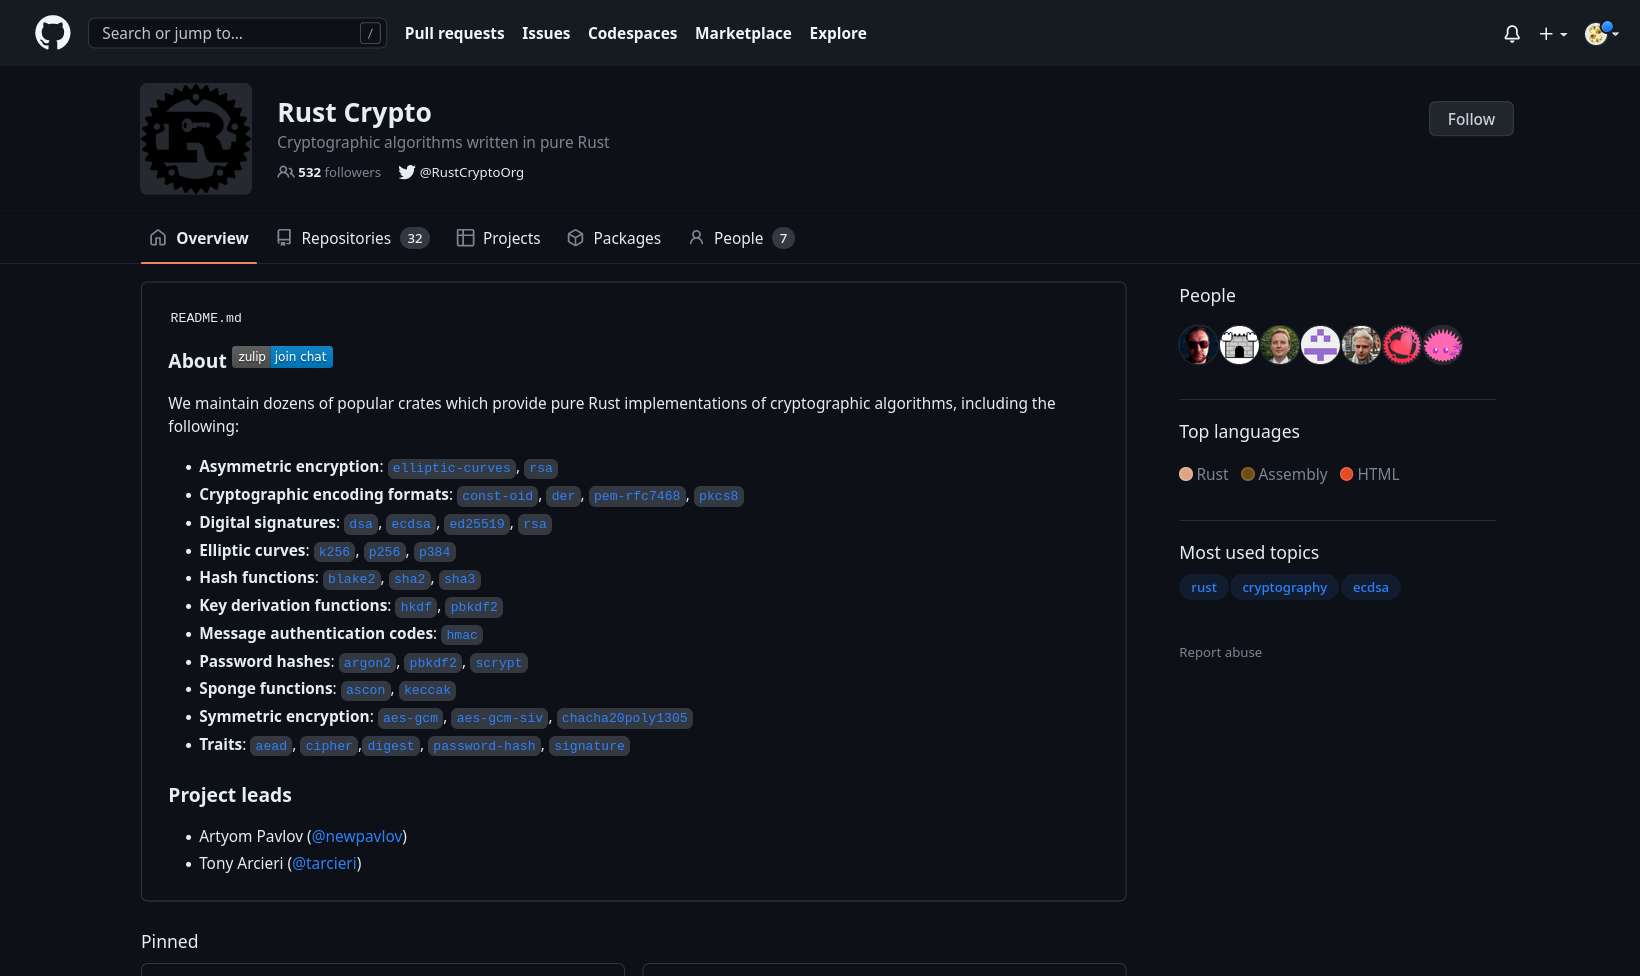
\includegraphics[width=\linewidth]{rust_crypto_github.png}
  \caption{RustCrypto's Github Organisation page}
  \label{fig:rc-github}
\end{figure}

\begin{figure}[H]
  \centering

  \begin{tikzpicture}
    % rug text items
    \node(Int) at (3, 10)  {\texttt{Integer}};
    \node(Rat) at (3, 9)   {\texttt{Rational}};
    \node(Flt) at (5.25, 10.04)  {\texttt{Float}}; % fuck knows, tikz hates me

    % rug boxes
    \node[inner sep=5pt, rounded corners, draw, fit=(Int) (Rat)] (gmp-items) {};
    \node[inner sep=5pt, rounded corners, draw, fit=(Flt)] (mpfr-items) {};
    \node[above right] at (gmp-items.north west) (rug-label) [] {\texttt{rug}};
    \node[above right] at (mpfr-items.north west) {\texttt{rug}};
    \node[inner sep=5pt, rounded corners, draw, fit=(gmp-items) (mpfr-items) (rug-label)] (rug) {};
    \node[above right, yshift=0.1cm] at (rug.north west) (rust-label) [] {\texttt{Rust}};

    % num text items
    \node(BInt) at (9, 10)  {\texttt{BigInt}};
    \node(BRat) at (9, 9)   {\texttt{BigRational}};
    \node(BFlt) at (12, 10) {\texttt{BigFloat}};

    % num boxes
    \node[inner sep=5pt, rounded corners, draw, fit=(BInt) (BRat)] (num-items) {};
    \node[inner sep=5pt, rounded corners, draw, fit=(BFlt)] (astro-items) {};
    \node[above right] at (num-items.north west) (num-label) [] {\texttt{num}};
    \node[above] at (astro-items.north) (astro-label) [] {\texttt{astro-float}};
    \node[inner sep=5pt, rounded corners, draw,
      fit=(num-items) (astro-items) (num-label) (astro-label)] (num) {};

    \begin{scope}[on background layer]
      \node[inner sep=5pt, rounded corners, draw, fill=rust, fit=(rug) (num) (rust-label)] (rust) {};
    \end{scope}

    % C libraries
    \node(GMP) at (3, 6) {\texttt{GNU GMP}};
    \node(MPFR) at (5.25, 6) {\texttt{GNU MPFR}};

    \node[inner sep=3pt, rounded corners, draw, fit=(GMP)] (gmp-box) {};
    \node[inner sep=3pt, rounded corners, draw, fit=(MPFR)] (mpfr-box) {};

    \node[above right] at (gmp-box.north west) (c-label) [] {\texttt{C}};

    \begin{scope}[on background layer]
      \node[inner sep=5pt, rounded corners, draw, fill=c!70, fit=(gmp-box) (mpfr-box) (c-label)] (c-box) {};
    \end{scope}

    \draw[dashed] (1.7,7.6) -- (6.7,7.6) node[right] {FFI Boundary};
    \draw[<->,thick,>=latex] (gmp-items.south) -- (gmp-box.north);
    \draw[<->,thick,>=latex] (mpfr-items.south) -- (mpfr-box.north);
  \end{tikzpicture}

  \caption{Pure Rust library (\texttt{num+astro-float}) vs Rust wrapper library (\texttt{rug})}
  \label{fig:pure-vs-wrapper}
\end{figure}

